\documentclass{article}

% if you need to pass options to natbib, use, e.g.:
%     \PassOptionsToPackage{numbers, compress}{natbib}
% before loading neurips_2019

% ready for submission
\usepackage[nonatbib]{neurips_2019_ml4ad}

% to compile a preprint version, e.g., for submission to arXiv, add add the
% [preprint] option:
% \usepackage[preprint, nonatbib]{neurips_2019_ml4ad}

% to compile a camera-ready version, add the [final] option, e.g.:
% \usepackage[final]{neurips_2019_ml4ad}

% to avoid loading the natbib package, add option nonatbib:
% \usepackage[nonatbib]{neurips_2019_ml4ad}

\usepackage[utf8]{inputenc} % allow utf-8 input
\usepackage[T1]{fontenc}    % use 8-bit T1 fonts
\usepackage{hyperref}       % hyperlinks
\usepackage{url}            % simple URL typesetting
\usepackage{booktabs}       % professional-quality tables
\usepackage{amsfonts}       % blackboard math symbols
\usepackage{nicefrac}       % compact symbols for 1/2, etc.
\usepackage{microtype}      % microtypography

% Custom packages
\usepackage[round]{natbib}
\usepackage{amsmath}
\usepackage{amssymb}
\usepackage{graphicx}
\usepackage{array, makecell}
\usepackage{tikz}
\usepackage{xspace}
\usepackage{float}
\usetikzlibrary{arrows,automata}
\usepackage{pgfplots}
\usetikzlibrary{intersections}
\usepackage{subcaption}
\usepackage[flushleft]{threeparttable}
\usepackage{cases}
\usepackage{multirow}



%%%%%%%%%%%%%%%%%%%%%%%%%%%%
% Paper dependent stuff    %
%%%%%%%%%%%%%%%%%%%%%%%%%%%%

\newcommand{\MLPC}{\texttt{MLP/Coordinates}\xspace}
\newcommand{\MLPG}{\texttt{MLP/Grid}\xspace}
\newcommand{\EgoAtt}{\texttt{Ego-Attention}\xspace}


%%%%%%%%%%%%%%%%%%%%%%%%%%%%
% Aesthetics               %
% over-underline, hat, bold%
%%%%%%%%%%%%%%%%%%%%%%%%%%%%

\newcommand{\eps}{\varepsilon}
\newcommand{\vareps}{\varepsilon}
\renewcommand{\epsilon}{\varepsilon}
%\renewcommand{\hat}{\widehat}
\renewcommand{\tilde}{\widetilde}
\renewcommand{\bar}{\overline}

\newcommand*{\MyDef}{\mathrm{\tiny def}}
\newcommand*{\eqdefU}{\ensuremath{\mathop{\overset{\MyDef}{=}}}}% Unscaled version



\def\:#1{\protect \ifmmode {\mathbf{#1}} \else {\textbf{#1}} \fi}
\newcommand{\CommaBin}{\mathbin{\raisebox{0.5ex}{,}}}

\newcommand{\wt}[1]{\widetilde{#1}}
\newcommand{\wh}[1]{\widehat{#1}}
\newcommand{\wo}[1]{\overline{#1}}
\newcommand{\wb}[1]{\overline{#1}}

% bf and bm missing due to conflict!!
\newcommand{\bsym}[1]{\mathbf{#1}}
\newcommand{\bzero}{\mathbf{0}}
\newcommand{\ba}{\mathbf{a}}
\newcommand{\bb}{\mathbf{b}}
\newcommand{\bc}{\mathbf{c}}
\newcommand{\bd}{\mathbf{d}}
\newcommand{\be}{\mathbf{e}}
\newcommand{\bg}{\mathbf{g}}
\newcommand{\bh}{\mathbf{h}}
\newcommand{\bi}{\mathbf{i}}
\newcommand{\bj}{\mathbf{j}}
\newcommand{\bk}{\mathbf{k}}
\newcommand{\bl}{\mathbf{l}}
\newcommand{\bn}{\mathbf{n}}
\newcommand{\bo}{\mathbf{o}}
\newcommand{\bp}{\mathbf{p}}
\newcommand{\bq}{\mathbf{q}}
\newcommand{\br}{\mathbf{r}}
\newcommand{\bs}{\mathbf{s}}
\newcommand{\bt}{\mathbf{t}}
\newcommand{\bu}{\mathbf{u}}
\newcommand{\bv}{\mathbf{v}}
\newcommand{\bw}{\mathbf{w}}
\newcommand{\bx}{\mathbf{x}}
\newcommand{\by}{\mathbf{y}}
\newcommand{\bz}{\mathbf{z}}

\newcommand{\bA}{\mathbf{A}}
\newcommand{\bB}{\mathbf{B}}
\newcommand{\bC}{\mathbf{C}}
\newcommand{\bD}{\mathbf{D}}
\newcommand{\bE}{\mathbf{E}}
\newcommand{\bF}{\mathbf{F}}
\newcommand{\bG}{\mathbf{G}}
\newcommand{\bH}{\mathbf{H}}
\newcommand{\bI}{\mathbf{I}}
\newcommand{\bJ}{\mathbf{J}}
\newcommand{\bK}{\mathbf{K}}
\newcommand{\bL}{\mathbf{L}}
\newcommand{\bM}{\mathbf{M}}
\newcommand{\bN}{\mathbf{N}}
\newcommand{\bO}{\mathbf{O}}
\newcommand{\bP}{\mathbf{P}}
\newcommand{\bQ}{\mathbf{Q}}
\newcommand{\bR}{\mathbf{R}}
\newcommand{\bS}{\mathbf{S}}
\newcommand{\bT}{\mathbf{T}}
\newcommand{\bU}{\mathbf{U}}
\newcommand{\bV}{\mathbf{V}}
\newcommand{\bW}{\mathbf{W}}
\newcommand{\bX}{\mathbf{X}}
\newcommand{\bY}{\mathbf{Y}}
\newcommand{\bZ}{\mathbf{Z}}

% calligraphic
\newcommand{\cf}{\mathcal{f}}
\newcommand{\cA}{\mathcal{A}}
\newcommand{\cB}{\mathcal{B}}
\newcommand{\cC}{\mathcal{C}}
\newcommand{\cD}{\mathcal{D}}
\newcommand{\cE}{\mathcal{E}}
\newcommand{\cF}{\mathcal{F}}
\newcommand{\cG}{\mathcal{G}}
\newcommand{\cH}{\mathcal{H}}
\newcommand{\cI}{\mathcal{I}}
\newcommand{\cJ}{\mathcal{J}}
\newcommand{\cK}{\mathcal{K}}
\newcommand{\cL}{\mathcal{L}}
\newcommand{\cM}{\mathcal{M}}
\newcommand{\cN}{\mathcal{N}}
\newcommand{\cO}{\mathcal{O}}
\newcommand{\cP}{\mathcal{P}}
\newcommand{\cQ}{\mathcal{Q}}
\newcommand{\cR}{\mathcal{R}}
\newcommand{\cS}{\mathcal{S}}
\newcommand{\cT}{\mathcal{T}}
\newcommand{\cU}{\mathcal{U}}
\newcommand{\cV}{\mathcal{V}}
\newcommand{\cW}{\mathcal{W}}
\newcommand{\cX}{\mathcal{X}}
\newcommand{\cY}{\mathcal{Y}}
\newcommand{\cZ}{\mathcal{Z}}

%%%%%%%%%%%%%%%%%%%%%%%%%%%%
% Math jargon              %
%%%%%%%%%%%%%%%%%%%%%%%%%%%%
\newcommand{\wrt}{w.r.t.\xspace}
\newcommand{\defeq}{\stackrel{\mathclap{\normalfont\mbox{\tiny def}}}{=}}
\newcommand{\maxund}[1]{\max\limits_{#1}}
\newcommand{\supund}[1]{\text{sup}\limits_{#1}}
\newcommand{\minund}[1]{\min\limits_{#1}}
\renewcommand{\epsilon}{\varepsilon}
\newcommand{\bigotime}{\mathcal{O}}


\DeclareMathOperator*{\argmin}{arg\,min} 
\DeclareMathOperator*{\argmax}{arg\,max} 
\DeclareMathOperator*{\cupdot}{\mathbin{\mathaccent\cdot\cup}}
\newcommand{\eqdef}{\buildrel \text{def}\over =}

%%%%%%%%%%%%%%%%%%%%%%%%%%%%
% Matrix operators         %
%%%%%%%%%%%%%%%%%%%%%%%%%%%%
\newcommand{\transpose}{^\mathsf{\scriptscriptstyle T}}
\newcommand{\transp}{\mathsf{\scriptscriptstyle T}}

%%%%%%%%%%%%%%%%%%%%%%%%%%%%
% Statistic operators      %
%%%%%%%%%%%%%%%%%%%%%%%%%%%%
\newcommand{\probability}[1]{\mathbb{P}\left(#1\right)}
\newcommand{\probdist}{Pr}
\DeclareMathOperator*{\expectedvalue}{\mathbb{E}}
\DeclareMathOperator*{\variance}{\text{Var}}
\newcommand{\expectedvalueover}[1]{\expectedvalue\limits_{#1}}
\newcommand{\condbar}{\;\middle|\;}
\newcommand{\gaussdistr}{\mathcal{N}}
\newcommand{\uniformdistr}{\mathcal{U}}
\newcommand{\bernoullidist}{\mathcal{B}}

%%%%%%%%%%%%%%%%%%%%%%%%%%%%
% Algebraic Sets           %
%%%%%%%%%%%%%%%%%%%%%%%%%%%%
\newcommand{\Real}{\mathbb{R}}
\newcommand{\Natural}{\mathbb{N}}
\newcommand{\statespace}{\mathcal{X}}
\newcommand{\funcspace}{\mathcal{F}}
\newcommand{\dynaspace}{\mathcal{T}}


\newtheorem{theorem}{Theorem}
\newtheorem{definition}{Definition}
\newtheorem{lemma}{Lemma}
\newtheorem{proposition}{Proposition}
\newtheorem{remark}{Remark}
\newtheorem{property}{Property}
\newtheorem{assumption}{Assumption}
\newtheorem{conjecture}{Conjecture}

\title{Social Attention for Autonomous Decision-Making in Dense Traffic}

% The \author macro works with any number of authors. There are two commands
% used to separate the names and addresses of multiple authors: \And and \AND.
%
% Using \And between authors leaves it to LaTeX to determine where to break the
% lines. Using \AND forces a line break at that point. So, if LaTeX puts 3 of 4
% authors names on the first line, and the last on the second line, try using
% \AND instead of \And before the third author name.

%Happy Horizontal People Transporter
%From the Sirius Cybernetics Corporation with a Genuine People Personality

\author{%
  Edouard Leurent\thanks{Equal contribution.} \\
  SequeL team, INRIA Lille -- Nord Europe\\
  Renault Group, France\\
  \texttt{edouard.leurent@inria.fr} \\
   \And
  Jean Mercat$^*$ \\
  Laboratoire des signaux et des syst\`emes, Centrale-Sup\'elec\\
  Renault Group, France\\
  \texttt{jean.mercat@renault.com} \\
}

\begin{document}
	
	
	\tikzset{
		state/.style={
			rectangle,
			draw=black, very thick,
			minimum height=2em,
			inner sep=2pt,
			text centered,
		},
		name plot/.style={every path/.style={name path global=#1}}
	}
	
	\pgfmathdeclarefunction{dnorm}{2}{%
		\pgfmathparse{1/(#2*sqrt(2*pi))*exp(-((x-#1)^2)/(2*#2^2))}%
	}
	

\maketitle

\begin{abstract}
  This work addresses the design of learning architectures for behavioural planning in a dense traffic setting. We claim that three important requirements are: dealing with a varying number of nearby vehicles, being invariant to the ordering chosen to describe them, while staying accurate and compact. We observe that the two most popular representations in the literature do not fit all these criteria, and show that they perform badly on an intersection-crossing task that involves complex anticipation and negotiation skills. In contrast, we propose an attention-based architecture that enjoys all these properties while also accounting for the existing interactions between the traffic participants. We show that this architecture leads to significant improvements in performance, and that it is able to capture interactions patterns that can be visualized and qualitatively interpreted.
\end{abstract}

\section{Introduction}

In the last decades, the problem of \emph{behavioural planning} -- that is, high-level decision-making in the context of autonomous driving -- has arguably received less attention and seen less progress than the other components of the typical robotics pipeline: perception and control \citep{Gonzalez2016}. Indeed, the vast majority of existing systems still rely on hand-crafted rules encoded as Finite State Machines \citep{Paden2016}. As a result, only a narrow set of specified use-cases are addressed as these methods cannot scale to more complex scenes, especially when the decision-making process involves interacting with other human drivers whose behaviours are uncertain and difficult to model explicitly.

This observation has led the community to turn to learning-based methods, which bear the promise of leveraging data to automatically learn a complex driving policy. In the imitation learning approach, a policy can be trained in a supervised manner to imitate human driving decisions \citep[e.g.][]{Pomerleau1989, Ross2011, Bojarski2016, Xu2016, Eraqi2017, Codevilla2017, Rehder2017c, Rezagholiradeh2018, Rhinehart2018, Bansal2018, Rhinehart2019}. Because the cost of human driving data collection at large scale can be prohibitive, another promising approach is train a policy in simulation using reinforcement learning \citep[e.g.][]{Cardamone2009, Ross2011, Mukadam2017, Chen2017, Isele2017, Isele2018, Ha2018, Kendall2019}.

Beyond the choice of reinforcement learning algorithm, the formalization of the problem as a Markov Decision Process plays an important part in the design of the system. Indeed, the definition of the state space involves choosing a representation of the driving scene. In this work, we focus in on how the vehicles are represented. In particular, we claim that the two most-widely used representations both suffer from different drawbacks: on the one hand, the \emph{list of features} representation is compact and accurate but has a varying-size and depends on the choice of ordering. On the other hand, the \emph{spatial grid} representation addresses these concerns but in return suffers from an accuracy-size trade-off.

Our contributions are the following: first, we propose an attention-based architecture for decision-making involving social interactions. This architecture allows to satisfy the variable-size and permutation invariance requirements even when using a \emph{list of features} representation. It also naturally accounts for interactions between the ego-vehicle and any other traffic participant.
Second, we evaluate our model on a challenging intersection-crossing task involving up to 15 vehicles perceived simultaneously. We show that our proposed method provides significant quantitative improvements, and that it enables to capture interaction patterns in a way that is visually interpretable.

\section{Background and Related Work}

\label{sec:background}

\paragraph{Model-free deep reinforcement learning} Reinforcement Learning is a general framework for sequential decision-making under uncertainty. It frames the learning objective as the optimal control of a Markov Decision Process $(S, A, P, R, \gamma)$ with measurable state space $S$, action space $A$, unknown reward function $R\in\Real^{S \times A}$, and unknown dynamics $P\in \cM(S)^{S \times A}$, where $\cM(\mathcal{X})$ denotes the probability measures over a set $\mathcal{X}$. The objective is to find a policy $\pi\in\cM(A)^S$ with maximal expected $\gamma$-discounted cumulative reward, called the value function $V^\pi$. Formally,

\begin{align*}
V^\pi(s) &\eqdef \expectedvalue\left[\sum_{t=0}^\infty \gamma^t R(s_t, a_t)\condbar s_0=s, a_t\sim \pi(a_t|s_t), s_{t+1}\sim P(s_{t+1}|s_t, a_t)\right]\\
Q^\pi(s, a) &\eqdef R(s, a) + \gamma \expectedvalueover{s'\sim P(s'|s, a)} V^\pi(s')
\end{align*}

The optimal action-value function $Q^* =  \max_\pi Q^\pi(s)$ satisfies the Bellman Optimality Equation \citep{bellman}:
\begin{equation*}
Q^*(s, a) = (\cT Q^*) (s, a) \eqdef \expectedvalueover{s'\sim P(s'|s, a)} \max_{a'\in A} \left[R(s, a) + \gamma Q^*(s', a')\right]
\end{equation*}

As $Q^*$ is a fixed-point of the Bellman Operator $\cT$ -- which is a contraction --, it can be computed by applying $\cT$ iteratively in a fixed-point iteration fashion. The \emph{Q-learning} algorithm \citep{Watkins} follows this procedure by applying a sampling version $\cT$ to a batch of collected experience. When dealing with a continuous state space $S$, we need to employ function approximation in order to generalise to nearby states. The \emph{Deep Q-Network} (DQN) algorithm \citep{Mnih2015} implements this idea by using a neural network model to represent the action-value function $Q$.

\paragraph{State-representation for social interactions}

In order to apply a reinforcement learning algorithm such as DQN to an autonomous driving problem, a state space $S$ must first be chosen, that is, a representation of the scene. When social interactions are relevant to the decision, the state should at leat compose a description of every nearby vehicle. A vehicle driving on a road can be described in the most general way by it's continuous position, heading and velocity. Then, the joint state of a road traffic with one ego-vehicle denoted $s_0$ and $N$ other vehicles can be described by the (unordered) set of individual vehicle states:

\begin{equation}
s = \left\lbrace s_i \right\rbrace_{i \in [0, N]}\qquad
\text{where}\qquad
s_i = \begin{bmatrix}
x_i & y_i & v^x_i & v^y_i & \cos\psi_i & \sin \psi_i
\end{bmatrix}^T
\label{eq:coordinates}
\end{equation}


\begin{figure}[tp]
	\centering
	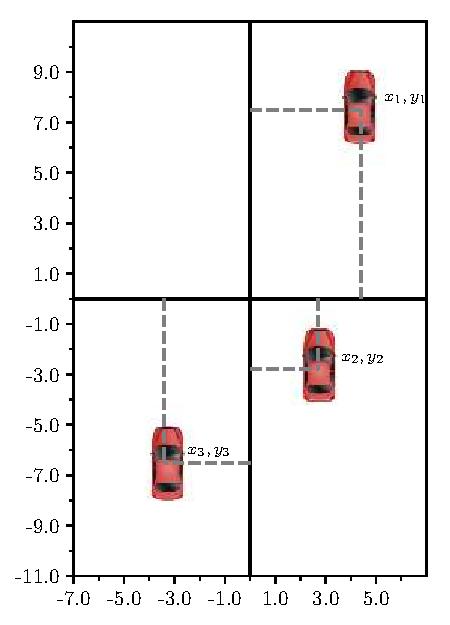
\includegraphics[width=0.25\textwidth]{img/coordinates}
	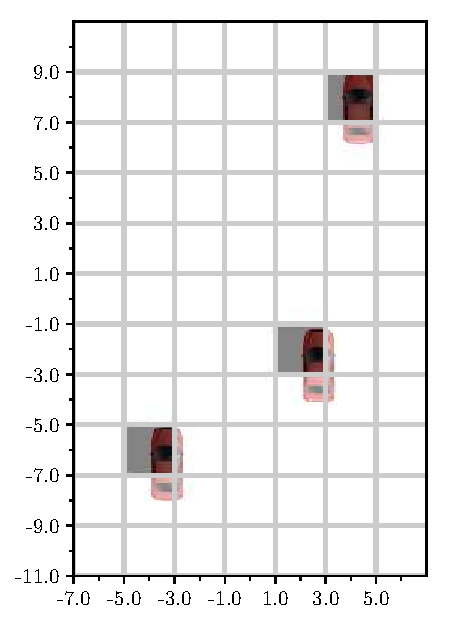
\includegraphics[width=0.25\textwidth]{img/map}
	\caption{The \emph{list of features} (left) and \emph{spatial grid} (right) representations}
	\label{fig:representation}
\end{figure}

This representation, that we call \emph{list of features}, is illustrated in \autoref{fig:representation} (left) and was used for instance in \citep{Bai2015, Gindele2015, Song2016, Sunberg2017, Paxton2017, Galceran2017, Chen2017}.


This encoding is efficient in the sense that it uses the smallest quantity of information necessary to represent the scene. However, it lacks two important properties. First, its size varies with the number of vehicles which can be problematic for the sake of function approximation which often expects constant-sized inputs. Second, we expect a driving policy $\pi$ to be \emph{permutation invariant}, i.e. not to be dependent on the order in which other traffic participants are listed. Ideally, this property should be enforced and not approximated by relying on the coverage of the $N!$ possible permutations $\tau$ of any given traffic state. Formally, we require that:
\begin{equation*}
\pi(\cdot|(s_0, s_1,\dotsc,s_N)) = \pi(\cdot|(s_0, s_{\tau(1)},\dotsc,s_{\tau(N)})) \quad\quad\quad \forall\tau \in \mathfrak{S}_N
\end{equation*}

A popular way to address this limitations is to use a \emph{spatial grid} representation. Instead of explicitly representing spatial information as variables $x, y$ along with other features $f$ directly inside the state $\{s_i=(x_i,y_i,f_i)\}_{i\in[0,N]}$ indexed on the vehicles, they are instead represented implicitly through the layout of several feature variables $f_{ij}$ organized in a tensor structure, where the $(i,j)$ indexes refer to the cells of a quantization of the 2D-space. This representation is illustrated in \autoref{fig:representation} (right). Note that the size of this tensor is related to the area covered divided by the length of the quantization, which reflects a trade-off between accuracy and dimensionality.
In an occupancy grid, the $f$ features contains presence information (0-1) and additional channels such as velocity and heading, as in \citep[e.g.][]{Isele2017, Fridman2018, Bansal2018, Rehder2017c}. Another example is the use of top-view RGB images \citep[e.g.][]{Bagnell2010, Rehder2017, Rehder2017c, Liu2018}.


This permutation invariance property can also be implemented within the policy architecture. A general technique to achieve this is to treat each entity similarly in the early stages -- e.g. through weight sharing -- before reducing them with a projection operator that is itself invariant to permutations, for instance a max-pooling as in \citep{Chen2017} or an average as in \citep{Qi2016}. A particular instantiation of this idea is attention mechanisms.


\paragraph{Attention mechanisms} {The attention architecture was introduced to enable neural networks to discover inter-dependencies within a variable number of inputs.
It has been used for pedestrian trajectory forecasting in~\cite{Vemula2018} with spatiotemporal graphs and in~\cite{Sadeghian2019CVPR} with spatial and social attention using a generative neural network. In~\cite{Sadeghian2018ECCV}, attention over top-view road scene images for car trajectory forecasting is used. Multi-head attention mechanism has been developed in~\cite{Vaswani2017} for sentence translation. In~\cite{Messaoud2019} a mechanism called non-local multi-head attention is developed. However, this is a spatial attention that does not allow vehicle-to-vehicle attention. In the present work, we use a multi-head social attention mechanism to capture vehicle-to-ego dependencies and build varying input size and permutation invariance into the policy model.}

\section{Model Architecture}
\label{sec:architecture}

Out of a complex scene description, the model should be able to filter information and consider only what is relevant for decision. In other words, the agent should \emph{pay attention} to vehicles that are close or conflict with the planned route. 

The proposed architecture is presented in \autoref{fig:architecture}. It is used to represent the $Q$-function that will be optimized by the DQN algorithm. It is composed of a first linear encoding layer whose weights are shared between all vehicles. At that point, the embeddings only contain individual features of size $d_x$. They are then fed to an ego-attention layer, composed of several heads stacked together. Such an attention head is illustrated in \autoref{fig:ego-attention}, and works in the following way: in order to select a subset of vehicles depending on the context, the ego-vehicle  first emits a query $Q = [q_0]\in\Real^{1 \times d_k}$, computed with a linear projection $L_q\in\Real^{d_x \times d_k}$ of its embedding. This query is then compared to a set of keys $K = [k_0, \dots, k_N]\in\Real^{N \times d_k}$ containing descriptive features $k_i$ for each vehicle, again computed with a shared linear projection $L_k\in\Real^{d_x \times d_k}$. The similarity between the query $q_0$ and any key $k_i$ is assessed by their dot product $q_0 k_i^T$. These similarities are then scaled by the inverse-square-root-dimension $1/\sqrt{d_k}$\footnote{This scaling is due to the fact that the dot-product of two independent random vectors with mean 0,  variance 1, and dimension $d_k$, is a random variable with mean 0 and variance $d_k$} and normalized with a softmax function $\sigma$ across vehicles. We obtain a stochastic matrix called the \emph{attention matrix}, which is finally used to gather a set of output value $V = [v_0, \dots, v_N]$, where each value $v_i$ is a feature computed with a shared linear projection $L_v\in\Real^{d_x \times d_v}$. Overall, the attention computation for each head can be written as:
\begin{equation}
\text{output}=\underbrace{\sigma\left(\frac{QK^T}{\sqrt{d_k}}\right)}_{\text{attention matrix}}V
\label{eq:selfattention}
\end{equation}
The outputs from all heads are finally combined with a linear layer, and the resulting tensor is then added to the ego encoding as in residual networks. We can easily see that this process is permutation invariant: indeed, a permutation $\tau$ will change the order of the rows in keys $K$ and values $V$ in \eqref{eq:selfattention} but will keep their correspondence. The final result is a dot product of values and key-similarities, which is independent of the ordering.


\begin{figure}[tp]
	\centering
	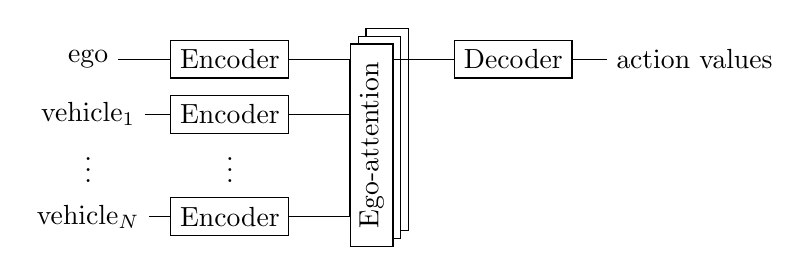
\begin{tikzpicture}
	\node(X1){ego};
	\node[below of=X1, node distance=0.7cm](X2){vehicle$_{1}$};
	\node[below of=X2, node distance=0.6cm](X3){$\vdots$};
	\node[below of=X3, node distance=0.7cm](X4){vehicle$_{N}$};
	
	\node[draw, right of=X1, node distance=1.8cm, rectangle](ENC1){Encoder};
	\node[draw, right of=X2, node distance=1.8cm, rectangle](ENC2){Encoder};
	\node[below of=ENC2, node distance=0.6cm](ENC3){$\vdots$};
	\node[draw, right of=X4, node distance=1.8cm, rectangle](ENC4){Encoder};
	
	\path (X1) edge (ENC1);
	\path (X2) edge (ENC2);
	\path (X4) edge (ENC4);
	

	\node[draw, rectangle, right of=ENC1, node distance=2.0cm, below=-0.4cm, fill=white](TRANS3){\rotatebox{90}{ Ego-attention }};
	\node[draw, rectangle, right of=ENC1, node distance=1.9cm, below=-0.3cm, fill=white](TRANS2){\rotatebox{90}{ Ego-attention }};
	\node[draw, rectangle, right of=ENC1, node distance=1.8cm, below=-0.2cm, fill=white](TRANS1){\rotatebox{90}{ Ego-attention }};
	
	\draw (ENC1.east) -| (TRANS1.west);
	\draw (ENC2.east) -| (TRANS1.west);
	\draw (ENC4.east) -| (TRANS1.west);
	
	
	\node[draw, right of=ENC1, node distance=3.6cm, rectangle](DEC1){Decoder};
	
	\draw (TRANS1.east) |- (DEC1.west);

	\node[right of=DEC1, node distance=2.3cm](Y1){action values};
	
	\draw (DEC1.east) -- (Y1.west);
	\end{tikzpicture}
	\caption{Block diagram of our model architecture. It is composed of several linear identical encoders, a stack of ego-attention heads, and a linear decoder.}
	\label{fig:architecture}
	
\end{figure}

\begin{figure}[tp]
	\centering
	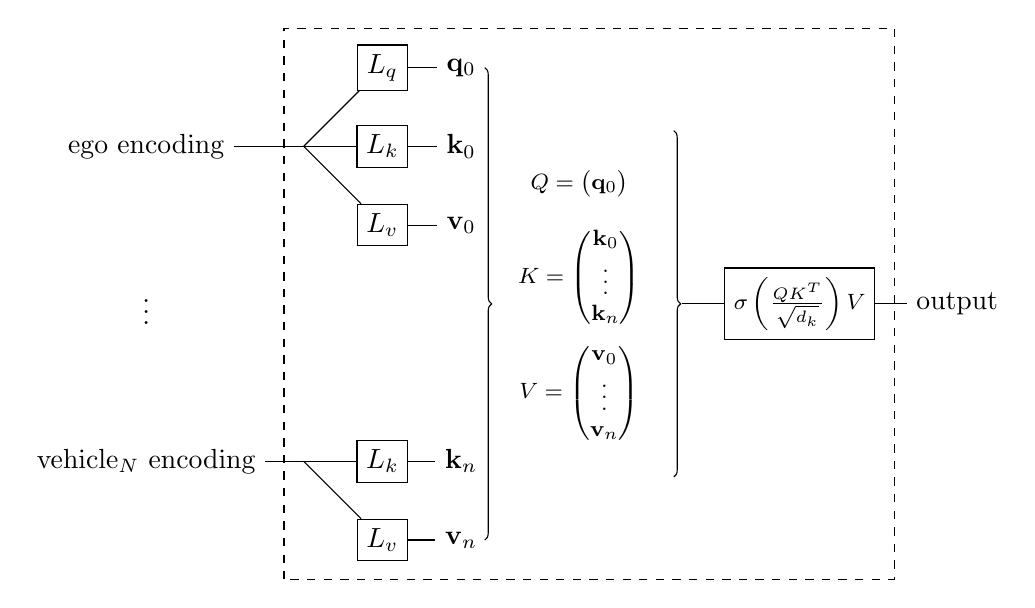
\begin{tikzpicture}[scale=1, every node/.style={scale=1}]
	\node(X1){ego encoding};
	\node[below of=X1, node distance=2cm](X2){$\vdots$};
	\node[below of=X2, node distance=2cm](X3){vehicle$_{N}$ encoding};
	
	\coordinate[right of= X1, node distance=2cm](X1b){};
	
	\draw (X1) -- (X1b);
	
	\node[draw, right of=X1b, node distance=1cm](LK1){$L_{k}$};
	\node[draw, below of=LK1, node distance=1cm](LV1){$L_{v}$};
	\node[draw, above of=LK1, node distance=1cm](LQ1){$L_{q}$};
	
	\draw (X1b) -- (LQ1);
	\draw (X1b) -- (LK1);
	\draw (X1b) -- (LV1);
	

	\node[right of=LQ1, node distance=1cm](Q1){$\mathbf{q}_0$};
	\node[right of=LK1, node distance=1cm](K1){$\mathbf{k}_0$};
	\node[right of=LV1, node distance=1cm](V1){$\mathbf{v}_0$};
	
	\draw (LQ1) -- (Q1);
	\draw (LK1) -- (K1);
	\draw (LV1) -- (V1);
	
	\coordinate[right of= X3, node distance=2cm](X3b){};
	
	\draw (X3) -- (X3b);
	
	\node[draw, right of=X3b, node distance=1cm](LK3){$L_{k}$};
	\node[draw, below of=LK3, node distance=1cm](LV3){$L_{v}$};

	\draw (X3b) -- (LK3);	
	\draw (X3b) -- (LV3);
	
	\node[right of=LK3, node distance=1cm](K3){$\mathbf{k}_{n}$};
	\node[right of=LV3, node distance=1cm](V3){$\mathbf{v}_{n}$};

	\draw (LK3) -- (K3);
	\draw (LV3) -- (V3);
	
	\coordinate[right of=Q1, node distance=0.3cm](TOP){};
	\coordinate[right of=V3, node distance=0.3cm](BOT){};
	\draw[decorate,decoration={brace}] (TOP) -- node[left=5pt]{} (BOT);
	
	\node[right of=X2, text width=3cm, node distance=5.5cm](EQ){
		\footnotesize \[Q = \left( \begin{matrix}
		\mathbf{q}_0
		\end{matrix} \right)\]
		\\
		\footnotesize \[K = \left( \begin{matrix}
		\mathbf{k}_0 \\
		\vdots \\
		\mathbf{k}_{n}
		\end{matrix} \right)\]
		\\
		\footnotesize \[ V = \left( \begin{matrix}
		\mathbf{v}_0 \\
		\vdots \\
		\mathbf{v}_{n}
		\end{matrix}\right) \]
	};

	\node[draw, right of=X2, node distance=8.3cm](EQ2){
	\footnotesize $\sigma\left(\frac{QK^T}{\sqrt{d_k}}\right)V$};

	\coordinate[left of=EQ2, node distance=1.6cm, above=2.2cm](TOP2){};
	\coordinate[left of=EQ2, node distance=1.5cm, below=0.0cm](MID2){};
	\coordinate[left of=EQ2, node distance=1.6cm, below=2.2cm](BOT2){};
	\draw[decorate,decoration={brace}] (TOP2) -- node[left=5pt]{} (BOT2);
	\draw (MID2) -- (EQ2);
	
	\node[right of=EQ2, node distance=2cm](OUT){output};
	\draw (EQ2) -- (OUT);
	
	\draw[draw=black, dashed] (1.75cm, -5.5cm) rectangle (9.5cm,1.5cm);
	\end{tikzpicture}
	\caption{Architecture of an ego-attention head.
		The blocks $L_{q}$, $L_{k}$, $L_{v}$ are linear layers. The keys $K$ and values $V$ are concatenated from all vehicles, while the query $Q$ is only produced by the ego-vehicle.}
	\label{fig:ego-attention}
\end{figure}


\section{Experiments}
\paragraph{Environment}

In this application, we use the \href{https://github.com/eleurent/highway-env}{highway-env} environment \citep{highway-env} for simulated highway driving and behavioural decision-making. We propose a new task where vehicle-to-vehicle interaction plays a significant part: crossing a four-way intersection.
The scene -- composed of two roads crossing perpendicularly -- is populated with several traffic participants initialized with random positions, velocities, and destinations. As in \citep{highway-env}, these vehicle are simulated with the Kinematic Bicycle Model, their lateral control is achieved by a low-level steering controller tracking a target route, and their longitudinal behaviour follows the Intelligent Driver Model. However, this model only considers same-lane interactions and special care was required to prevent lateral collisions at the intersection. To that end, we implemented the following simplistic behaviour: each vehicle predicts the future positions of its neighbours over a three-second horizon by using a constant velocity model. In case of predicted collision with a neighbour, the yielding vehicle is determined based on road priorities, and must brake until the collision prediction ceases. 

In this context, the agent must drive a vehicle by controlling its acceleration chosen from a finite set of actions $A = \{\texttt{SLOWER}, \texttt{NO-OP}, \texttt{FASTER}\}$. The lateral control is performed automatically by a low-level controller, such that the problem complexity is focused on the high-level interactions with other vehicles, namely the decision to either yield or take way. The agent is rewarded by $1$ when it drives at maximum velocity, $0$ otherwise, and by $-5$ when a collision occurs.

\paragraph{Agents}

We evaluate three different agents, whose characteristics are summarized in \autoref{tab:agents}.
\begin{itemize}
	\item \MLPC: a \emph{list of features} state representation is used, as described in Section \ref{sec:background}. The model is a simple multi-layer perceptron (MLP). Because this architecture requires a fixed-size input, we use zero-padding to fill the input tensor up to a maximum number $N=14$ of observed vehicles, and add an additional \emph{presence} feature to the coordinates described in \eqref{eq:coordinates} so as to identify active rows.
	\item \MLPG: a \emph{spatial grid} representation is used, as described in Section \ref{sec:background}, with a $11 \times 11$ grid where each cell represents a $5\text{m}\times 5$m square. The model is a multi-layer perceptron.
	\item \EgoAtt: a \emph{list of features} state representation is used along with the Ego-Attention architecture described in Section \ref{sec:architecture}. As this model supports varying-size inputs, zero-padding is not required.
\end{itemize}

\begin{table}[tp]
	\centering
	\begin{threeparttable}
		\caption{Characteristics of the agents}
		\label{tab:agents}
		\begin{tabular}{lccc}
			\toprule
			Architecture & \MLPC & \MLPG & \EgoAtt \\
			\midrule 
			Input sizes & [15, 7] & [11, 11, 5] & [1-15, 7] \\
			Layers sizes & [128, 128] &  [48, 48] & \makecell[tl]{Encoder: [64, 64] \\Attention: 2 heads, $d_k=32$ \\ Decoder: [64, 64]} \\
			Number of parameters & 3.0e4 & 3.2e4 & 3.4e4 \\
			Variable input size & No & No &  {Yes}  \\
			Permutation invariant & No & {Yes} &  {Yes} \\
			\bottomrule
		\end{tabular}
	\end{threeparttable}
\end{table}

These agents are all trained with the DQN algorithm using the same hyperparameters, and their architectures are scaled to admit about the same number of trainable parameters for fair comparison.

\paragraph{Performances}

We plot in \autoref{fig:results} the evolution of the total reward, episode length and average velocity during training, over 4000 episodes and repeated across 120 random seeds.
The \MLPC agent learns to accelerate to earn short-term rewards, as shown by its high average velocity, but fails to exploit the information of other vehicles and crashes often, leading to shorter episodes. In short, we obtain a risky and blind policy that is the worst performing.
Conversely, the \MLPG architecture benefits from its invariance to permutations and manages to learn to brake upon arrival at the intersection to avoid collisions, as we can see from its higher episode length. However, it only proceeds when the intersection has been fully cleared, as reflected by its low average velocity. This results in an overly cautious policy -- a common trait colloquially known as the \emph{freezing robot problem} \citep{Trautman2010} -- but a slight increase in performance.
In stark contrast, the \EgoAtt policy quickly learns both when it must slow down at the intersection but also when it can exploit the gaps in the traffic and take way to vehicles that are far/slow enough. The overall resulting behaviour is qualitatively more nuanced and human-like.

\begin{figure}[htp]
	\centering
	\begin{subfigure}[t]{.75\linewidth}
		\centering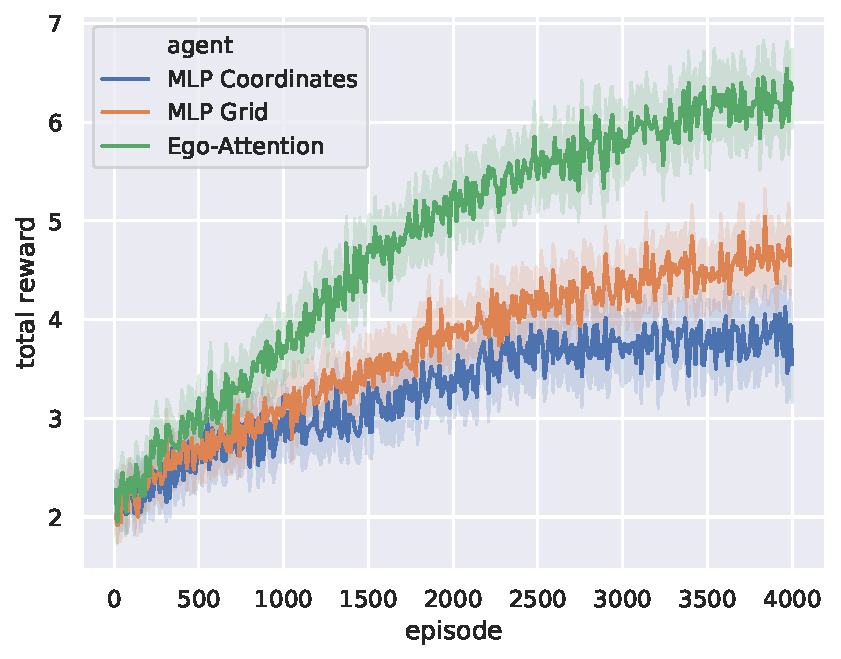
\includegraphics[width=\linewidth]{img/total_reward}
	\end{subfigure}
\\
	\begin{subfigure}[t]{.49\linewidth}
		\centering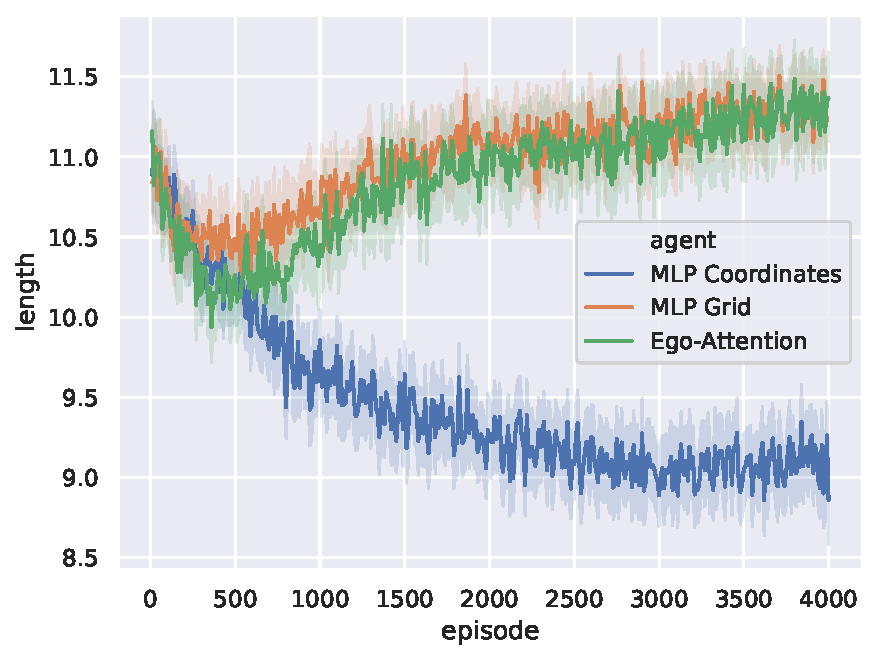
\includegraphics[width=\linewidth]{img/length}
	\end{subfigure}
	\begin{subfigure}[t]{.49\linewidth}
		\centering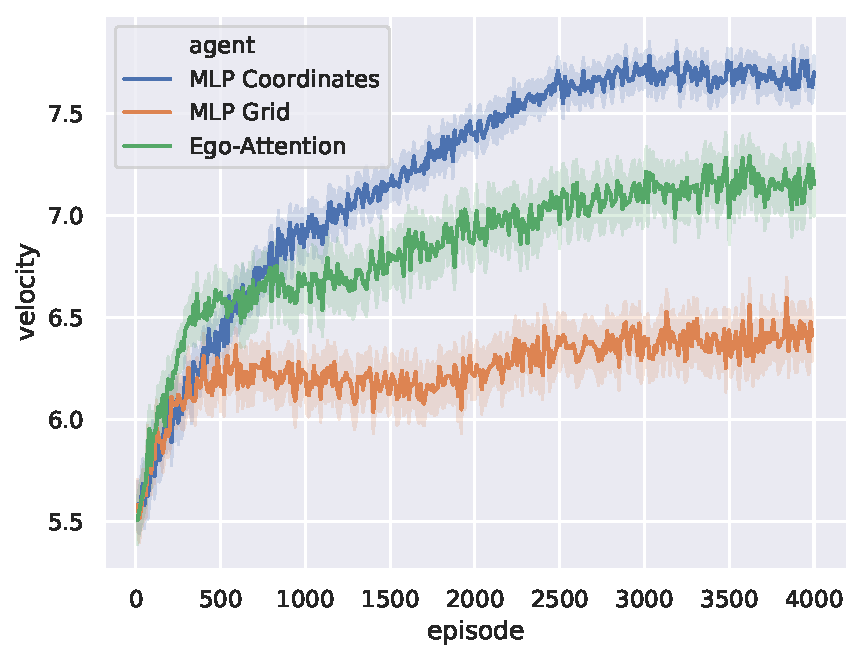
\includegraphics[width=\linewidth]{img/velocity}
	\end{subfigure}
%	\begin{subfigure}[t]{.49\linewidth}
%	\centering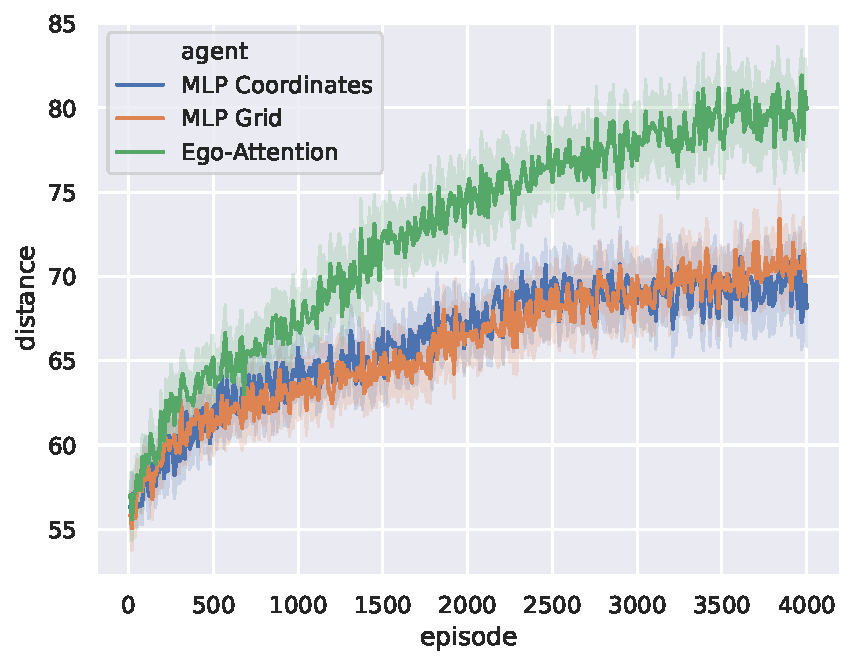
\includegraphics[width=\linewidth]{img/distance}
 %   \end{subfigure}
 \caption{The episode total rewards, lengths, and average velocity (higher is better). We display the mean values -- along with their 95\% confidence interval -- averaged over 120 random seeds.}
 \label{fig:results}
\end{figure}

\paragraph{Attention interpretation}

This model is also more interpretable, as we can visualize the learnt attention matrix.

TODO: figure yield vs take way

Additional videos are available at \url{http://url.github.io}

\paragraph{Exploiting interaction patterns}
The priority rules are note enforced through rewards but interactions: based on the defined road priorities, some vehicles will take way to the ego-vehicle, while others will not.

change the priority -> influences the rules of interactions -> changes the learnt behaviour.
By switching the priority road, the resulting policy changes: In the exact same initial state, the ego-vehicle takes way to incoming vehicles when its policy was trained on a priority road, and gives way otherwise. The only change between these two situations is the rules of interactions imposed on simulated vehicles, which showcases the ability of our proposed architecture to discover and exploit such interaction patterns.


\section{Conclusion}

TODO

%\subsubsection*{Acknowledgments}
%
%TODO

\bibliographystyle{named}
\bibliography{references}




\end{document}
